\chapter{Geração do mapa}

A posição do robô no mapa em cada instante é representada por um ponto no plano cartesiano e por um ângulo, que indica para qual sentido o robô está orientado. Esse ponto no plano indica onde está o centro de movimento do robô, que é o ponto médio entre as duas rodas.

Neste projeto, a determinação do deslocamento do robô é determinada primariamente pelos encoders presentes cada roda. O acelerômetro e o giroscópio são utilizados para aumentar a confiabilidade dos cálculos de deslocamento, principalmente em caso de escorregamento das rodas.

Na próxima seção será explicada a teoria da determinação do deslocamento, velocidade e aceleração do centro de movimento do robô a partir das leituras dos encoders em cada instante. Na seção \ref{sec:teoria_acel_giro} será explicitada a forma como as leituras do acelerômetro e giroscópio serão utilizadas para aumentar a confiabilidade das medições.

Na Figura \ref{fig:robo} está presente um esquema básico do robô visto de cima e virado com a frente para a direita. Na figura estão presentes os nomes das variáveis que são utilizadas nos cálculos posteriores. As medidas $R$, $R_D$ e $R_E$ representam os raios de um movimento circular uniforme descrito pelo robô, supondo que e roda esquerda esteja se deslocando mais do que a direita. Esse aspecto será melhor explicado nas seções seguintes. 

\begin{figure}[H]
  \centering
  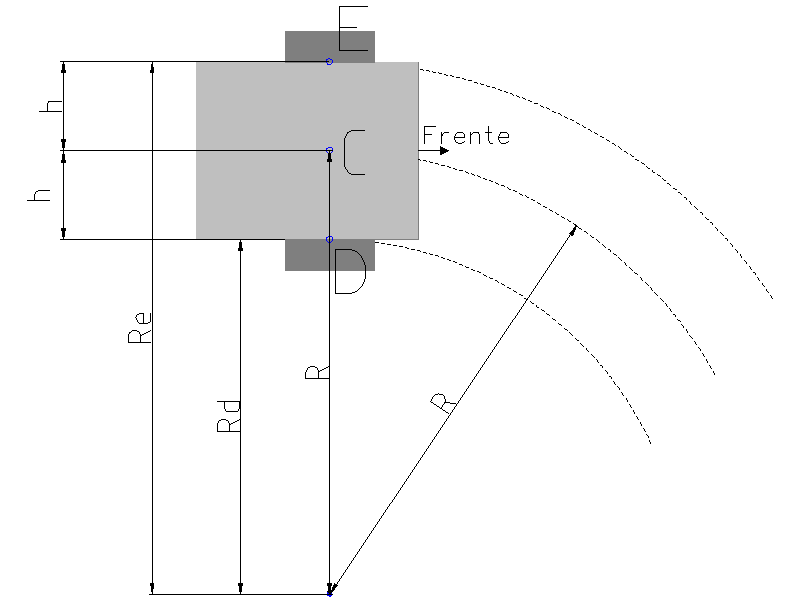
\includegraphics[width=0.8\textwidth, keepaspectratio]{./figuras/robo/robo.png}
  \caption{Representação básica do robô em movimento circular uniforme (visão superior).}
  \label{fig:robo}
\end{figure}

Um aspecto importante a ressaltar é que o sistema de coordenadas do Processing (a biblioteca usada para desenhar o mapa 2D na interface gráfica) possui o eixo Y invertido. Portanto, os ângulos crescem no sentido horário, e não no anti-horário como seria o convencional. Essa convenção do Processing (ângulos que crescem em sentido horário) foi utilizada integralmente neste projeto.

\section{Encoders}

Há dois dados importantes a determinar sobre o deslocamento do centro de movimento do robô: o deslocamento linear (distância absoluta percorrida) e o angular (variação do ângulo de orientação do robô). Cada encoder fornece uma medida de contagem de pulsos por volta a cada intervalo de amostragem. 

Na Figura \ref{fig:roda_encoder} está presente um representação básica de uma roda, acoplada a um encoder. Os números da figura são utilizados como índices nos cálculos explicitados posteriormente.

\begin{figure}[H]
  \centering
  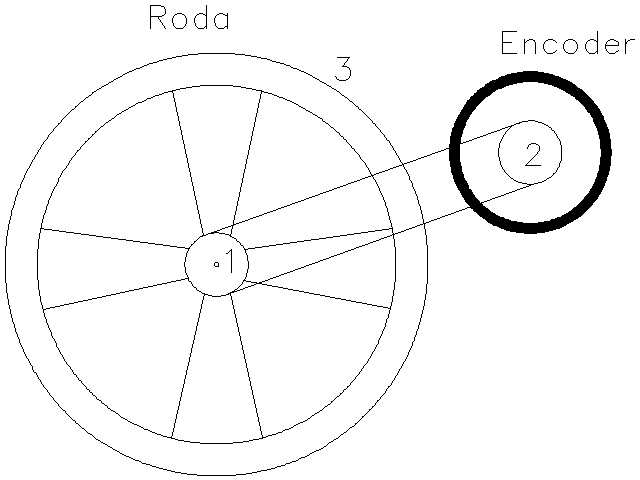
\includegraphics[width=0.5\textwidth, keepaspectratio]{./figuras/robo/roda_encoder.png}
  \caption{Representação de uma roda acoplada a um encoder.}
  \label{fig:roda_encoder}
\end{figure}

\subsection{Deslocamento de cada roda}

Um princípio importante utilizado nos cálculos é a relação entre o deslocamento $\Delta x$ ao redor de uma circunferência (de raio $R$) e a variação do ângulo $\Delta \theta$:

\begin{equation}
  \Delta x = R \cdot \Delta \theta
  \label{eq:deslocamento_circunferencia}
\end{equation}

Nos cálculos a seguir, faz-se uso do índice 1 para o eixo da roda, 2 para o eixo do encoder e 3 para a própria roda, de acordo com a figura \ref{fig:roda_encoder}. Para determinar a distância percorrida pela roda, deve-se considerar a circunferência do eixo da roda ($C_1$), a circunferência do eixo do encoder ($C_2$) e a circunferência da roda ($C_3$).

O acoplamento do eixo do encoder com o eixo da roda é feita por uma correia de borracha, e portanto considera-se que o deslocamento ($ \Delta x_1$) na superfície do eixo da roda é igual ao deslocamento ($ \Delta x_2$) na superfície do eixo do encoder. Pode-se, com isso, calcular:

\begin{eqnarray*}
   \Delta x_1 =  \Delta x_2 \rightarrow \Delta \theta_1 R_1 = \Delta \theta_2 R_2 \rightarrow \Delta \theta_1 \frac{C_1}{2 \pi} = \Delta \theta_2 \frac{C_2}{2 \pi} 
\end{eqnarray*}

\begin{equation}
  \Delta \theta_1 = \frac{C_2}{C_1} \cdot \Delta \theta_2
  \label{eq:theta1_theta2}
\end{equation}

Calculando-se a relação entre a contagem de pulsos do encoder ($E$) e o ângulo de rotação ($\Delta \theta_2$) do eixo do encoder, levando-se em conta que há uma contagem de 1800 pulsos por volta:

\begin{equation}
  \Delta \theta_2 = \frac{2 \pi}{1800} \cdot E \unit{rad}
  \label{eq:E_theta2}
\end{equation}

Substituindo-se a equação \ref{eq:E_theta2} na \ref{eq:theta1_theta2}, tem-se que:

\begin{equation}
  \Delta \theta_1 = \frac{C_2}{C_1} \frac{2 \pi}{1800} \cdot E \unit{rad}
  \label{eq:theta_1}
\end{equation}

Calculando-se a relação entre a variação do ângulo do eixo da roda ($\Delta \theta_1$) e o deslocamento da roda ($x_3$):

\begin{eqnarray*}
  \Delta \theta_1 = \Delta \theta_3 \rightarrow \Delta \theta_1 =  \Delta x_3 R_3 \rightarrow \Delta \theta_1 = \Delta x_3 \frac{C_3}{2 \pi} \rightarrow  \Delta x_3 = \Delta \theta_1 \frac{2 \pi}{C_3}
\end{eqnarray*}

Substituindo-se o valor de ($\Delta \theta_1$) da equação \ref{eq:theta_1}:

\begin{eqnarray*}
   \Delta x_3 = \frac{C_2}{C_1} \frac{2 \pi}{1800} \cdot E \cdot \frac{2 \pi}{C_3} = \frac{C_2}{C_1 C_3} \frac{(2 \pi)^2}{1800} \cdot E
\end{eqnarray*}

\begin{empheq}[box=\fbox]{equation}
   \Delta x_3 = \frac{C_2}{C_1 C_3} \frac{\pi^2}{450} \cdot E
  \label{eq:x_3}
\end{empheq}


Que é o valor do deslocamento da roda em função da contagem de pulsos do encoder. 


\subsection{Deslocamento do centro de movimento do robô}

Como já explicitado anteriormente, o centro de movimento do robô considerado é o ponto médio entre as duas rodas. As duas variáveis para determinar em cada instante de tempo são o deslocamento linear (distância absoluta percorrida) e o angular (variação do ângulo de orientação do robô). Considerando-se que em cada instante o robô descreve um movimento circular uniforme (MCU), o raio da trajerória deve ser determinado para que os cálculos de posicionamento do robô possam ser feitos. Este raio depende do deslocamento das rodas em cada instante, e é uma importante variável que será estudada na próxima subseção.

Nos cálculos que serão explicitados a seguir, utiliza-se o índice E para a roda esquerda, C para o centro de movimento do robô e D para a roda direita.

Uma relação importante a notar a princípio é que a variação do ângulo de orientação em cada instante é igual nos três pontos: E (roda esquerda), C (centro de movimento) e D (roda direita), visto que todos estão fixos em relação à carcaça do robô. Parte-se da seguinte relação fundamental, portanto:

\begin{equation}
  \Delta \theta_E = \Delta \theta_D = \Delta \theta_C
  \label{eq:relacao_fundamental_theta}
\end{equation}



\subsubsection{Raio do movimento circular uniforme}

Para determinar o raio ($R$) descrito pelo centro de movimento do robô em sua trajetória instantânea em MCU, usa-se os dois primeiros termos da igualdade da equação \ref{eq:relacao_fundamental_theta}:

\begin{eqnarray*}
  \Delta \theta_E = \Delta \theta_D \rightarrow \frac{\Delta x_E}{R_E} = \frac{\Delta x_D}{R_D} 
\end{eqnarray*}

Sabe-se, pela Figura \ref{fig:robo}, que:
\begin{equation*}
  R_E = R + h, ~ ~ R_D = R - h
\end{equation*}

Portanto:

\begin{eqnarray*}
  \frac{\Delta x_E}{R + h} = \frac{\Delta x_D}{R - h} ~\rightarrow~ \frac{\Delta x_E}{\Delta x_D} = \frac{R + h}{R - h} ~\rightarrow~ \frac{\Delta x_E (R - h)}{\Delta x_D} = R + h 
\end{eqnarray*}
\begin{eqnarray*}
  \frac{\Delta x_E \cdot R - \Delta x_E \cdot h}{\Delta x_D} = R + h ~\rightarrow~ 
  \frac{\Delta x_E}{\Delta x_D} \cdot R - \frac{\Delta x_E}{\Delta x_D} \cdot h = R + h ~\rightarrow~ 
  \frac{\Delta x_E}{\Delta x_D} \cdot R - R = \frac{\Delta x_E}{\Delta x_D} \cdot h + h
\end{eqnarray*}
\begin{eqnarray*}
  R \left( \frac{\Delta x_E}{\Delta x_D} - 1 \right) = h \left( \frac{\Delta x_E}{\Delta x_D} + 1 \right) ~\rightarrow~
  R = h \cdot \frac{\left( \frac{\Delta x_E}{\Delta x_D} + 1 \right)}{\left( \frac{\Delta x_E}{\Delta x_D} - 1 \right)}  ~\rightarrow~
  R = h \cdot \frac{\frac{\Delta x_E + \Delta x_D}{x_D}}{\frac{\Delta x_E - \Delta x_D}{\Delta x_D}} 
\end{eqnarray*}

\begin{empheq}[box=\fbox]{equation}
  R = h \cdot \frac{\Delta x_E + \Delta x_D} {\Delta x_E - \Delta x_D}
  \label{eq:R}
\end{empheq}

Vê-se que o raio $R$ do movimento circular uniforme em cada instante depende do deslocamento de cada roda ($\Delta x_E$ e $\Delta x_D$) e da distãncia $h$ entre as rodas e o centro de movimento do robô.


\subsubsection{Deslocamento linear} 

Para calcular o deslocamento linear do centro de movimento do robô, usa-se os dois últimos termos da equação \ref{eq:relacao_fundamental_theta}. Vale ressaltar que poderiam ser escolhidos também o primeiro e o último termos, pois o resultado obtido seria idêntico. Tem-se que:

\begin{eqnarray*}
  \Delta \theta_D = \Delta \theta_C \rightarrow \frac{\Delta x_D}{R_D} = \frac{\Delta x_C}{R} 
\end{eqnarray*}

Mas:
\begin{equation*}
  R_D = R - h
\end{equation*}

Portanto:
\begin{eqnarray*}
  \frac{\Delta x_D}{R - h} = \frac{\Delta x_C}{R} ~\rightarrow~ x_D = x_C \cdot \frac{R - h}{R} 
\end{eqnarray*}

Substituindo-se o valor de $R$ da equação \ref{eq:R}:
\begin{eqnarray*}
  \Delta x_D = \Delta x_C \left[ \frac{h \cdot \frac{\Delta x_E + \Delta x_D}{\Delta x_E - \Delta x_D} - h}{h \cdot \frac{\Delta x_E + \Delta x_D}{\Delta x_E - \Delta x_D}} \right]
\end{eqnarray*}

Dividindo-se o numerador e denominador do segundo termo por $h$:
\begin{equation*}
  \Delta x_D = \Delta x_C \left[ \frac{\frac{\Delta x_E + \Delta x_D}{\Delta x_E - \Delta x_D} - 1}{\frac{\Delta x_E + \Delta x_D}{\Delta x_E - \Delta x_D}} \right]
\end{equation*}

Multiplicando-se o numerador e denominador do segundo termo por $\frac{\Delta x_E - \Delta x_D}{\Delta x_E + \Delta x_D}$:

\begin{equation*}
  \Delta x_D = \Delta x_C \left[1 - \frac{\Delta x_E - \Delta x_D}{\Delta x_E + \Delta x_D} \right] ~\rightarrow~
  \Delta x_D = \Delta x_C \left[\frac{(\Delta x_E + \Delta x_D) - (\Delta x_E - \Delta x_D)}{\Delta x_E + \Delta x_D} \right] 
\end{equation*}
\begin{equation*}
  \Delta x_D = \Delta x_C \cdot \left[ \frac{2 \Delta x_D}{\Delta x_E + \Delta x_D} \right] ~\rightarrow~
  \Delta x_C = \frac{\Delta x_D}{\left(\frac{2 \Delta x_D}{\Delta x_E + \Delta x_D} \right)}
\end{equation*}

\begin{empheq}[box=\fbox]{equation}
  \Delta x_C = \frac{\Delta x_E + \Delta x_D}{2}
  \label{eq:desloc_linear}
\end{empheq}

Notas-se que o deslocamento linear do centro de movimento do robô ($\Delta x_C$) é uma média simples dos dois deslocamentos lineares das rodas. Vê-se que ele não depende do raio de deslocamento nem da distância entre as duas rodas.


\subsubsection{Deslocamento angular}

O deslocamento angular ($\Delta \theta_c$) do centro de movimento do robô em cada instante pode ser calculado a partir do deslocamento linear e do raio do movimento circular uniforme. Usando-se a relação da equação \ref{eq:deslocamento_circunferencia}, tem-se que:


\begin{empheq}[box=\fbox]{equation}
  \Delta \theta_c = \frac{\Delta x_C}{R}
  \label{eq:desloc_angular}
\end{empheq}


Onde $\Delta x_C$ é o deslocamento linear do robô (equação \ref{eq:desloc_linear}) e $R$ é o raio do movimento circular uniforme (equação \ref{eq:R}). 

\subsubsection{Casos especiais}

Há dois casos especiais que devem ser considerados no cálculo do deslocamento (a partir dos dados dos encoders) do centro de movimento do robo. O primeiro é quando as duas rodas têm deslocamento igual ($\Delta x_E = \Delta x_D$). O raio do movimento circular (equação \ref{eq:R}) neste caso é:

\begin{equation}
  R = h \cdot \frac{\Delta x_E + \Delta x_D} {\Delta x_E - \Delta x_D} = h \cdot \frac{2 \cdot \Delta x_E}{0} \rightarrow \infty
  \label{eq:caso_especial1_R}
\end{equation}


O raio tende a infinito, o que implica que o deslocamento angular (equação \ref{eq:desloc_angular}) seja:

\begin{equation}
  \Delta \theta_c = \frac{\Delta x_C}{R} = \frac{\Delta x_C}{\infty} \rightarrow 0
  \label{eq:caso_especial1_theta}
\end{equation}

Já o deslocamento linear (equação \ref{eq:desloc_linear}) é:

\begin{equation}
  \Delta x_C = \frac{\Delta x_E + \Delta x_D}{2} = \frac{2 \Delta x_E}{2} = \Delta x_E
  \label{eq:caso_especial1_x}
\end{equation}

Isso corresponde à realidade, uma vez que quando as rodas têm deslocamentos iguais o robô está se deslocando sem fazer curvas. Não há deslocamento angular, portanto, e o deslocamento linear do centro de movimento é igual ao deslocamento de cada roda.

O segundo caso especial ocorre quando os deslocamento têm módulos iguais, porêm sentidos contrários (ou seja, $\Delta x_E = - \Delta x_D$). O raio nesse caso é:

\begin{equation}
  R = h \cdot \frac{\Delta x_E + \Delta x_D} {\Delta x_E - \Delta x_D} = h \cdot \frac{\Delta x_E - \Delta x_E}{\Delta x_E + \Delta x_E} = 0
    \label{eq:caso_especial2_R}
\end{equation}


O deslocamento linear (equação \ref{eq:desloc_linear}) é:

\begin{equation}
  \Delta x_C = \frac{\Delta x_E + \Delta x_D}{2} = \frac{\Delta x_E - \Delta x_E}{2} = 0
  \label{eq:caso_especial2_x}
\end{equation}

Esse valor corresponde à realidade, pois quando as rodas se deslocam em sentidos contários, e na mesma quantidade, o centro de movimento do robô não se desloca linearmente, mas apenas muda seu ângulo.
Usando-se a equação \ref{eq:desloc_angular}, tenta-se calcular o valor do deslocamento angular:

\begin{equation}
  \Delta \theta_c = \frac{\Delta x_C}{R} = \frac{0}{0}
  \label{eq:caso_especial2_theta}
\end{equation}

O valor obtido é indeterminado quando usa-se essa equação. Porém, analisando-se a natureza deste caso especial, pode ser notado que há um movimento circular cujo centro é o ponto médio entre as rodas (que é o centro de movimento do robô). O raio do MCU é a distância $h$ entre uma roda e o centro do robô, e o deslocamento ao longo da circunferência é o deslocamento de qualquer uma uma das rodas. Portanto, a equação \ref{eq:deslocamento_circunferencia} pode ser utilizada, isolando-se a variável $\theta$, para determinar o deslocamento angular do robô:

\begin{equation}
  \Delta \theta_c = \frac{\Delta x_E}{h}
  \label{eq:caso_especial2_theta2}
\end{equation}

\subsubsection{Considerações sobre a notação utilizada}

A notação utilizada no decorrer do texto para representar o estado de uma variável em certo instante discreto de tempo é um número subscrito entre parênteses. Por exemplo, a posição $\overrightarrow{P}$ do robô em um instante de tempo $n$ é representado por:$\overrightarrow{P}_{(n)}$. 

Outro aspecto presente no decorrer do texto, que vale ser ressaltado para que haja melhor entendimento das demostrações, é o fato de que $\Delta x_{(n)}$ é o deslocamento absoluto do robô do intervalo de tempo discreto de $(n-1)$ até $n$.

%\begin{equation}
%  \Delta x_{(n)} = x_{(n)} - x_{(n - 1)}
%  \label{eq:delta_x}
%\end{equation}
%
%Sendo que $\Delta x_{(n)}$ é o deslocamento do robô do intervalo $(n-1)$ até $n$.

\subsubsection{Velocidade e aceleraçao}

A velocidade e aceleração lineares do centro de movimento do robô podem ser calculadas por derivação numérica do deslocamento e velocidade em cada intervalo de tempo. Em cada intervalo discreto $n$:

\begin{equation}
  v_{c (n)} = \frac{\Delta x_{c (n)} }{t_{(n)} - t_{(n-1)}}
  \label{eq:velocidade_encoders}
\end{equation}

\begin{equation}
  a_{c (n)} = \frac{v_{c (n)} - v_{c (n-1)}}{t_{(n)} - t_{(n-1)}}
  \label{eq:aceleracao_encoders}
\end{equation}


A velocidade e aceleração angulares podem ser também obtidas por derivação numérica, considerando-se que o raio do movimento circular uniforme do robô é constante dentro do intervalo considerado. Em cada intervalo discreto $n$:

\begin{equation}
  \omega_{c (n)} = \frac{\Delta \theta_{c (n)} }{t_{(n)} - t_{(n-1)}}
  \label{eq:omega_encoders}
\end{equation}

\begin{equation}
  \alpha_{c (n)} = \frac{\omega_{c (n)} - \omega_{c (n-1)}}{t_{(n)} - t_{(n-1)}}
  \label{eq:alpha_encoders}
\end{equation}


\section{Acelerômetro e giroscópio}
\label{sec:teoria_acel_giro}

O acelerômetro e o giroscópio são utilizados para aumentar a confiabilidade dos dados de deslocamento do robô em caso de escorregamento das rodas.



Como definido na seção \ref{sec:codificacao_mensagens}, é recebido um valor de 2 bytes para cada eixo do acelerômetro. A faixa de funcionamento do acelerômetro está configurada em $\pm 2$ g, logo a sensibilidade pelo \textit{datasheet} é de 16384 LSB/g. Portanto, o valor de aceleração pode ser obtido pela fórmula:

\begin{equation}
  a = \frac{valorMedido}{16384} \cdot g \unit{m/s^2}
  \label{eq:acel}
\end{equation}

Onde g é a aceleração da gravidade ($9,80665 \unit{m/s^2}$). 

Para cada eixo do giroscópio, também e obtido um valor de 2 bytes. A faixa de funcionamento do giroscópio está configurada em $\pm 250$ graus/s, logo a sensibilidade pelo \textit{datasheet} é de 131 LSB/(graus/s). Portanto, o valor de velocidade angular pode ser obtida pela fórmula:

\begin{equation}
  \omega = \frac{valorMedido}{131} \unit{graus/s} = \frac{\pi}{180} \cdot \frac{valorMedido}{131} \unit{rad/s}
  \label{eq:giro}
\end{equation}


A princípio, apenas o eixo X do acelerômetro (voltado para a frente do robô) e o eixo Z do giroscópio (posicionado no sentido baixo/cima) serão utilizados para mapeamento, visto que os dados poderão ser dessa forma comparados facilmente com os dados obtidos pelos encoders. Os sensores serão posicionados no centro de movimento do robô (ponto médio entre as rodas) para realizar uma comparação de acelerações (encoders \textit{vs} acelerômetro) e velocidades angulares (encoders \textit{vs.} giroscópio).

Para determinar a velocidade e deslocamento lineares a partir dos dados do acelerômetro, efetua-se uma integração numérica (simples e dupla) da aceleração linear em cada intervalo discreto $n$:

\begin{equation}
  v_{(n)} = v_{(n - 1)} + a_{(n)} \cdot (t_{(n)} - t_{(n-1)})
  \label{eq:v_acelerometro}
\end{equation}
\begin{equation}
  \Delta x_{(n)} = v_{(n)} \cdot (t_{(n)} - t_{(n-1)})
  \label{eq:x_acelerometro}
\end{equation}

Para determinar o deslocamento angular a partir dos dados do giroscópio, efetua-se uma integração numérica (simples) da velocidade angular em cada intervalo discreto $n$:

\begin{equation}
  \Delta \theta_{(n)} = \Delta \theta_{(n - 1)} + \omega_{(n)} \cdot (t_{(n)} - t_{(n-1)})
  \label{eq:theta_giroscopio}
\end{equation}



\section{Sensores infra-vermelhos}

Os sensores infra-vermelhos são usados para detectar obstáculos próximos ao robô (de 30 a 150 cm de distância). Na Figura \ref{fig:robo_ir} está explicitada uma representação de um sensor infra-vermelho detectando um obstáculo. Na figura estão presentes os nomes das variáveis utilizadas nos cálculos. Como já explicado no começo do capítulo, o sistema de coordenadas do Processing (a biblioteca utilizada para desenhar o mapa 2D na interface gráfica) possui o eixo Y invertido. Portanto, os ângulos crescem no sentido horário e não no anti-horário como seria o convencional. Por essa razão, o ângulo ``-theta(n)'' da figura é negativo. 

\begin{figure}[H]
  \centering
  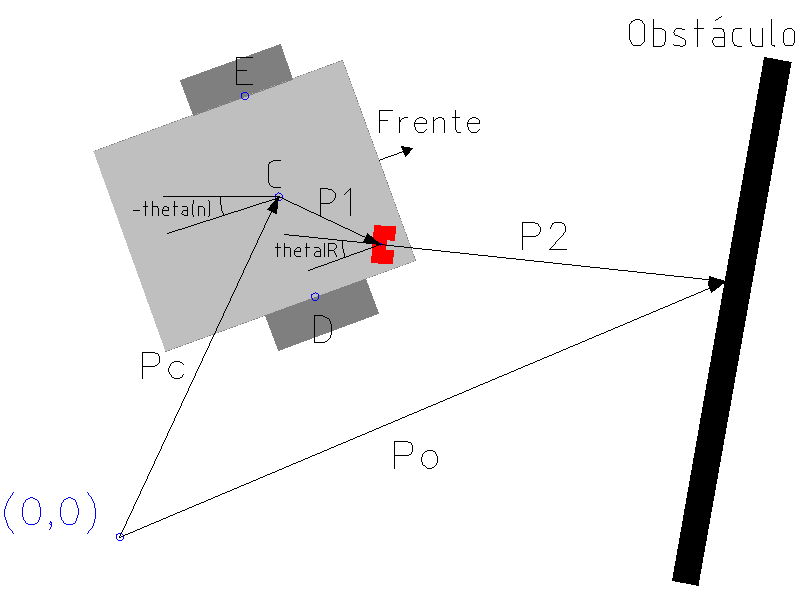
\includegraphics[width=0.8\textwidth, keepaspectratio]{./figuras/robo/robo_ir.png}
  \caption{Representação básica do robô e um sensor infra-vermelho detectando um obstáculo (visão superior).}
  \label{fig:robo_ir}
\end{figure}

Para obter a posição em que um obstáculo detectado está no mapa, primeiramente deve-se obter a distância entre o obstáculo e o sensor infra-vermelho. Como explicitado em \cite{bellator_2012}, o valor $x$ recebido em 1 byte do sensor pode ser convertido para a distãncia $d$ em centímetros pela fórmula (obtida por interpolação polinomial):

\begin{equation}
  d = 3,6404 \cdot 10^{-7} x^3 - 2,4435 \cdot 10^{-4} x^3 + 6,0732 \cdot 10^{-2} x^2 - 6,8962 x + 339,361
  \label{eq:IR_dist}
\end{equation}


Sendo $\overrightarrow{P_C}$ o vetor que sai da origem e vai até o centro de movimento do robô, $\overrightarrow{P_1}$ o vetor que vai do centro do robô até o sensor, e $\overrightarrow{P_2}$ o vetor que vai do sensor até o ponto do obstáculo detectado, faz-se a seguinte soma vetorial para encontrar o vetor $\overrightarrow{P_O}$, que é a posição do obstáculo no mapa:

\begin{equation}
  \overrightarrow{P_O} = \overrightarrow{P_C} + \overrightarrow{P_1} + \overrightarrow{P_2}
  \label{eq:IR_vector}
\end{equation}


O vetor $\overrightarrow{P_C}$ pode ser facilmente determinado de acordo com a equação abaixo. Sendo $\overrightarrow{P}_{(n)}$ a última posição do robô (intervalo discreto $n$):

\begin{equation}
  \overrightarrow{P_C} = \overrightarrow{P}_{(n)}
  \label{eq:IR-P_C}
\end{equation}

O vetor $\overrightarrow{P_1}$ é o vetor que vai do centro de movimento do robô até o sensor infra-vermelho (informação obtida das configurações iniciais do robô), rotacionado pelo ângulo em que o robô está na última posição. Sendo $\overrightarrow{P_{IR}}$ o vetor que vai do centro do robô até o sensor, e $\theta_{(n)}$ o ângulo em que o robô está orientado na última posição (intervalo discreto $n$):


\begin{equation}
  |\overrightarrow{P_1}| = |\overrightarrow{P_{IR}}|
  \label{eq:IR-P_1_modulo}
\end{equation}
\begin{equation}
  \phi \left\{ \overrightarrow{P_1} \right\} = \phi \left\{ \overrightarrow{P_{IR}} \right\} + \theta_{(n)}
  \label{eq:IR-P_1_fase}
\end{equation}


O vetor $\overrightarrow{P_2}$ é um vetor com magnitude igual à distância detectada pelo sensor, e ângulo igual a: ângulo relativo do sensor no robô (informação obtida das configurações iniciais) somado com o ângulo em que o robô está na última posição. Sendo $d$ a distãncia detectada pelo sensor infra-vermelho, $\theta_{IR}$ o ângulo em que o sensor infra-vermelho está posicionado no robô, e tendo $\theta_{(n)}$ o mesmo significado que na equação anterior:

\begin{equation}
  |\overrightarrow{P_2}| = d
  \label{eq:IR-P_2_modulo}
\end{equation}
\begin{equation}
  \phi \left\{ \overrightarrow{P_2} \right\} = \theta_{IR} + \theta_{(n)}
  \label{eq:IR-P_2_fase}
\end{equation}


%Em termos matemáticos:
%\begin{equation}
%  \overrightarrow{P_C} = \overrightarrow{P}
%  \label{eq:IR-P_C}
%\end{equation}
%\begin{eqnarray*}
%  |\overrightarrow{P_1}| &=&  \overrightarrow{P_{IR}}\\
%  \phi(\overrightarrow{P_1}) &=& \theta
%  \label{eq:IR-P_!}
%\end{eqnarray*}
%
\section{Algoritmo de posicionamento}

O algoritmo proposto para determinação da posição do robô em cada instante de tempo, utilizando os vários sensores (encoders, acelerômetro e giroscópio), está explicitado nesta seção. Para cada amostra dos sensores recebida, o algoritmo efetua os seguintes passos:

\begin{enumerate}
  \item A partir das leituras dos encoders ($\Delta x_E$ e $\Delta x_D$), usando as equações \ref{eq:desloc_linear} e \ref{eq:desloc_angular}, calcular deslocamento linear ($\Delta x_C$, em metros) e angular ($\Delta \theta_c$, em $rad$) do centro de movimento do robô.
  \item Derivar duas vezes o deslocamento linear ($\Delta x_C$), usando as equações \ref{eq:velocidade_encoders} e \ref{eq:aceleracao_encoders} para obter aceleração linear ($a_C$, em $m/s^2$), e derivar uma vez o deslocamento angular ($\theta_C$), usando a equação \ref{eq:omega_encoders}, para obter a velocidade angular ($\omega_C$, em $rad/s$).
  \item Comparar a aceleração linear ($a_C$) e a velocidade angular ($\omega_C$), obtidas com os encoders, com as leituras do acelerômetro ($a_a$) e giroscópio ($\omega_g$). Caso a diferença dos valores passe de um limite (determinado experimentalmente), é provável que um escorregamento de rodas tenha ocorrido.
  \item Baseado na comparação anterior, especificar pesos para a aceleração linear (encoders \textit{vs.} acelerômetro) e velocidade angular (encoders \textit{vs.} giroscópio), dando mais prioridade ao acelerômetro e giroscópio caso escorregamentos sejam detectados. Calcular com base nesses pesos a aceleração linear final ($a$) e a velocidade angular final ($\omega$).
  \item Usando-se as equações \ref{eq:v_acelerometro} e \ref{eq:x_acelerometro}, integrar duplamente a aceleração linear ($a$) para obter o deslocamento linear ($\bm{\Delta x}$) do robô, e a partir da equação \ref{eq:theta_giroscopio} integrar uma vez a velocidade angular ($\omega$) para obter o deslocamento angular ($\bm{\Delta \theta}$) do robô.
  \item A partir das equações \ref{eq:P_x} e \ref{eq:P_y} explicitadas abaixo, calcular a nova posição ($\overrightarrow{P}_{(n)}$) do robô, e a partir da equação \ref{eq:theta_n} calcular o novo ângulo $\theta_{(n)}$ do robô. Decompondo-se o vetor posição ($\overrightarrow{P}$) em suas componentes $P_x$ e $P_y$, tem-se que no intervalo discreto $n$:
    \begin{equation}
      P_{x (n)} = P_{x (n-1)} + \Delta x \cdot \cos{(\theta_{(n-1)})}
      \label{eq:P_x}
    \end{equation}
    \begin{equation}
      P_{y (n)} = P_{y (n-1)} + \Delta x \cdot \sin{(\theta_{(n-1)})}
      \label{eq:P_y}
    \end{equation}
    \begin{equation}
      \theta_{(n)} = \theta_{(n-1)} + \Delta \theta
      \label{eq:theta_n}
    \end{equation}
\end{enumerate}

%Nota-se que o acelerômetro e giroscópio entram em ação quando diferenças muito grandes entre os dados destes e dos encoders forem detectadas. As diferenças limites para que essa detecção ocorra são determinadas experimentalmente.

